\documentclass[letterpaper,11pt]{article}
\usepackage{listings}
\usepackage[pdftex]{graphicx} 
\usepackage[utf8]{inputenc}
%\usepackage[english]{babel}
\usepackage{alltt}
\usepackage{color}
\usepackage{url}
\usepackage[T1]{fontenc}
\usepackage{float}
\usepackage{hyperref}
\usepackage{longtable}
\usepackage{caption}
\usepackage{spverbatim}
\usepackage[table,xcdraw]{xcolor}
\usepackage{multirow}
\usepackage{amsmath}

\definecolor{dkgreen}{rgb}{0,0.6,0}
\definecolor{gray}{rgb}{0.5,0.5,0.5}
\definecolor{mauve}{rgb}{0.58,0,0.82}
\definecolor{codegreen}{rgb}{0,0.6,0}
\definecolor{codegray}{rgb}{0.5,0.5,0.5}
\definecolor{codepurple}{rgb}{0.58,0,0.82}
\definecolor{backcolour}{rgb}{0.95,0.95,0.92}

\addtolength{\textwidth}{4cm}
\addtolength{\hoffset}{-2cm}
\addtolength{\textheight}{4cm}
\addtolength{\voffset}{-2cm}

\lstdefinestyle{mystyle}{
    backgroundcolor=\color{backcolour},   
    commentstyle=\color{codegreen},
    keywordstyle=\color{magenta},
    numberstyle=\tiny\color{codegray},
    stringstyle=\color{codepurple},
    basicstyle=\footnotesize,
    breakatwhitespace=false,         
    breaklines=true,                 
    captionpos=b,                    
    keepspaces=true,                 
    numbers=left,                    
    numbersep=5pt,                  
    showspaces=false,                
    showstringspaces=false,
    showtabs=false,                  
    tabsize=2
}

\lstset{style=mystyle}

\lstset{
	basicstyle=\footnotesize,
	breaklines=true,
}

\title{Bibliography management: BibTeX}
\author{Share\LaTeX}

\begin{document}

\begin{titlepage}

\begin{center}

\Huge{Assignment 5}

\Large{CS834-F16:  Introduction to Information Retrieval}

\Large{Fall 2016}


\Large{Erika Siregar}

\vfill

% Bottom of the page
\Large{CS Department - Old Dominion University  \\ \today}


\end{center}

\end{titlepage}


\section*{Question 10.3}
\begin{spverbatim}
Compute five iterations of HITS (see Algorithm 3) and PageRank (see Figure 4.11) on the graph in Figure 10.3. Discuss how the PageRank scores compare to the hub and authority scores produced by HITS.
\end{spverbatim}

\subsection*{Answer}

Figure \ref{fig:10_3} shows the directed graph from the textbook \cite{Croft:2009:SEI:1516224} on which we will calculate the scores of HITS and PageRank. Computing HITS (authorities and hubs) and PageRank scores are pretty easy since we can just utilize the Link Analysis procedure that is provided by python library `networkx' \cite{networkx-hits-pagerank}. 

\begin{figure}[H]
	\fbox{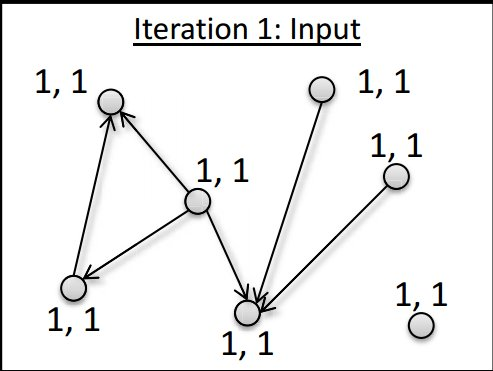
\includegraphics[scale=0.6]{10_3}}
	\centering
	\caption{Figure 10.3 from the textbook \cite{Croft:2009:SEI:1516224}}
	\label{fig:10_3}
\end{figure}

Figure \ref{fig:hits_pagerank} shows the scores of HITS (authorities and hubs) and PageRank, which are obtained by running the code in listing \ref{lst:10_3.py}. We only need to set the number of iterations. 

\begin{figure}[H]
	\fbox{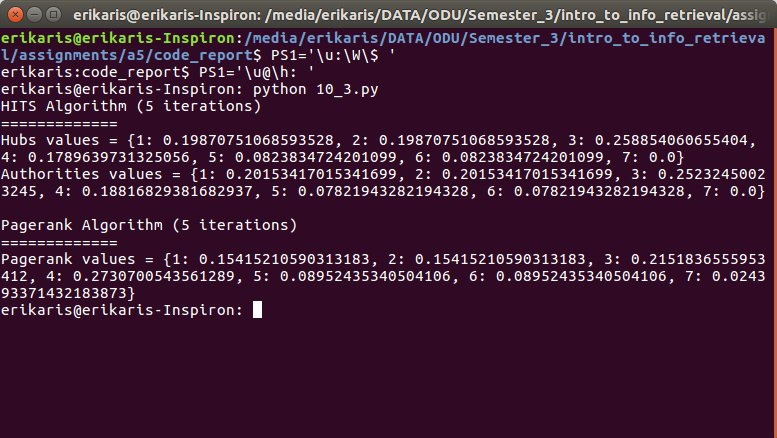
\includegraphics[scale=0.6]{hits_pagerank}}
	\centering
	\caption{HITS and Pagerank for Figure 10.3 with 5 Iterations}
	\label{fig:hits_pagerank}
\end{figure}

To make the analysis and comparison easier, I transformed the output int figure \ref{fig:hits_pagerank} into a neat table format as can be seen on table \ref{tab: hits_pagerank}. From table \ref{tab: hits_pagerank}, we can see that, generally, the authorities values are linearly proportional to those of PageRank. After 5 iterations, node 3 gets the highest score for `authorities' and the second highest score for `PageRank'. Nodes 1 and 2 get lower `authorities' score than that of node 3, but higher `authorities' score compare to nodes 5 and 6. The same thing can also be concluded by comparing the PageRank scores for those five nodes (1, 2, 3, 5, and 6). The strange thing happens on node 4, where its `authorities' score is lower than node 3, but its `PageRank' score is higher than node 3. This anomaly takes place probably because we only do 5 iterations. Maybe, if we continue iterating until the values converge into certain number, this anomaly will not happen. 

\begin{table}[h!]
	\centering
	\begin{tabular}{|l|l|l|l|}
		\hline
		\multicolumn{1}{|c|}{\multirow{2}{*}{\textbf{Node}}} & \multicolumn{3}{c|}{\textbf{Score}} \\ \cline{2-4} 
		\multicolumn{1}{|c|}{} & \multicolumn{1}{c|}{\textbf{Hubs}} & \multicolumn{1}{c|}{\textbf{Authorities}} & \multicolumn{1}{c|}{\textbf{PageRank}} \\ \hline
		1 & 0.198707510685935 & 0.201534170153416 & 0.154152105903131 \\ \hline
		2 & 0.198707510685935 & 0.201534170153416 & 0.154152105903131 \\ \hline
		3 & 0.258854060655404 & 0.252324500232450 & 0.215183655595341 \\ \hline
		4 & 0.178963973132505 & 0.188168293816829 & 0.273070054356128 \\ \hline
		5 & 0.082383472420110 & 0.078219432821943 & 0.089524353405041 \\ \hline
		6 & 0.082383472420110 & 0.078219432821943 & 0.089524353405041 \\ \hline
		7 & 0.000000000000000 & 0.000000000000000 & 0.024393371432184 \\ \hline
	\end{tabular}
	\caption{HITS and Pagerank for Figure 10.3 with 5 Iterations}
	\label{tab: hits_pagerank}
\end{table}

\begin{lstlisting}[language=python, caption={Computing HITS and PageRank}, label={lst:10_3.py}]
#!/usr/bin/python

import networkx as nx

def hits(G, iter=100, nstart=None, normalized=True):
if type(G) == nx.MultiGraph or type(G) == nx.MultiDiGraph:
raise Exception("hits() not defined for graphs with multiedges.")
if len(G) == 0:
return {},{}
# choose fixed starting vector if not given
if nstart is None:
h=dict.fromkeys(G,1.0/G.number_of_nodes())
else:
h=nstart
# normalize starting vector
s=1.0/sum(h.values())
for k in h:
h[k]*=s
i=0
while True: # power iteration: make up to max_iter iterations
if i >= iter: break

hlast=h
h=dict.fromkeys(hlast.keys(),0)
a=dict.fromkeys(hlast.keys(),0)
# this "matrix multiply" looks odd because it is
# doing a left multiply a^T=hlast^T*G
for n in h:
for nbr in G[n]:
a[nbr]+=hlast[n]*G[n][nbr].get('weight',1)
# now multiply h=Ga
for n in h:
for nbr in G[n]:
h[n]+=a[nbr]*G[n][nbr].get('weight',1)
# normalize vector
s=1.0/max(h.values())
for n in h: h[n]*=s
# normalize vector
s=1.0/max(a.values())
for n in a: a[n]*=s

i+=1
if normalized:
s = 1.0/sum(a.values())
for n in a:
a[n] *= s
s = 1.0/sum(h.values())
for n in h:
h[n] *= s
return h,a

def pagerank(G, alpha=0.85, personalization=None,
iter=100, nstart=None, weight='weight',
dangling=None):
if len(G) == 0:
return {}

if not G.is_directed():
D = G.to_directed()
else:
D = G

# Create a copy in (right) stochastic form
W = nx.stochastic_graph(D, weight=weight)
N = W.number_of_nodes()

# Choose fixed starting vector if not given
if nstart is None:
x = dict.fromkeys(W, 1.0 / N)
else:
# Normalized nstart vector
s = float(sum(nstart.values()))
x = dict((k, v / s) for k, v in nstart.items())

if personalization is None:
# Assign uniform personalization vector if not given
p = dict.fromkeys(W, 1.0 / N)
else:
missing = set(G) - set(personalization)
if missing:
raise nx.NetworkXError('Personalization dictionary '
'must have a value for every node. '
'Missing nodes %s' % missing)
s = float(sum(personalization.values()))
p = dict((k, v / s) for k, v in personalization.items())

if dangling is None:
# Use personalization vector if dangling vector not specified
dangling_weights = p
else:
missing = set(G) - set(dangling)
if missing:
raise nx.NetworkXError('Dangling node dictionary '
'must have a value for every node. '
'Missing nodes %s' % missing)
s = float(sum(dangling.values()))
dangling_weights = dict((k, v/s) for k, v in dangling.items())
dangling_nodes = [n for n in W if W.out_degree(n, weight=weight) == 0.0]

# power iteration: make up to max_iter iterations
for _ in range(iter):
xlast = x
x = dict.fromkeys(xlast.keys(), 0)
danglesum = alpha * sum(xlast[n] for n in dangling_nodes)
for n in x:
# this matrix multiply looks odd because it is
# doing a left multiply x^T=xlast^T*W
for nbr in W[n]:
x[nbr] += alpha * xlast[n] * W[n][nbr][weight]
x[n] += danglesum * dangling_weights[n] + (1.0 - alpha) * p[n]

return x

if __name__ == '__main__':
iter = 5
G = nx.Graph()

# Add 7 nodes
G.add_nodes_from(range(1,8))

# Add 6 edges
G.add_edges_from([(1,2), (3,1), (3,2), (3,4), (5,4), (6,4)])

# Compute hubs and authorities normalized values using hits
h, a = hits(G, iter=iter)

print 'HITS Algorithm ({} iterations)'.format(iter)
print '============='
print 'Hubs values = {}'.format(h)
print 'Authorities values = {}'.format(a)
print ''

# Compute pagerank of each nodes
pr = pagerank(G, iter=iter)

print 'Pagerank Algorithm ({} iterations)'.format(iter)
print '============='
print 'Pagerank values = {}'.format(pr)

\end{lstlisting}



\noindent\makebox[\linewidth]{\rule{\textwidth}{0.4pt}}

\section*{Question 10.5}
\begin{spverbatim}
Find a community-based question answering site on the Web and ask two questions, one that is low-quality and one that is high-quality. Describe the answer quality of each question.
\end{spverbatim}

\subsection*{Answer:}
For this assignment, I asked 2 questions on 2 different comunity-based question answering site. For the low-quality question, I asked about \textbf{\textit{`What is the purpose of our life?'}}\footnote{https://answers.yahoo.com/question/index?qid=20161216122515AAPvTIw\&page=4} on Yahoo Answers \url{https://answers.yahoo.com/} as can be seen on figure \ref{fig:10_5_q}. For the high-quality question, I asked the question \textbf{\textit{`BUILD-MAX-HEAP running time for array sorted in decreasing order'}} on Stackoverflow \footnote{http://stackoverflow.com/questions/39691923/build-max-heap-running-time-for-array-sorted-in-decreasing-order} as can be seen on figure \ref{fig:10_5_a1}.

\begin{figure}[H]
	\fbox{
\includegraphics[scale=0.5]{10_5_q}}
	\centering
	\caption{Low Quality Question I asked on Yahoo Answers}
	\label{fig:10_5_q}
\end{figure}

\begin{figure}[H]
	\fbox{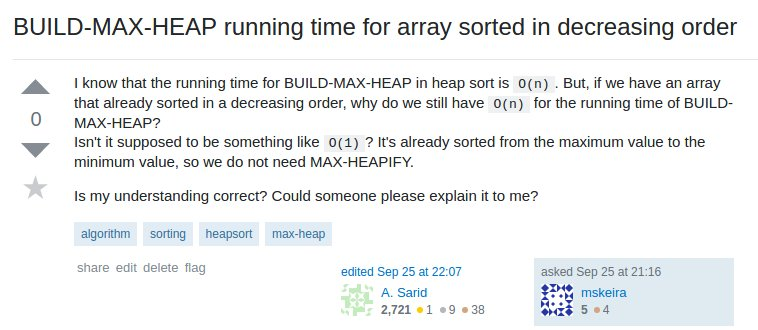
\includegraphics[scale=0.5]{10_5_hi_quality}}
	\centering
	\caption{High Quality Question I asked on Stackoverflow}
	\label{fig:10_5_hi_quality}
\end{figure}

By the time I write this report, I got 37 answers for the low-quality question on Yahoo Answers. Some of the answers can be seen on figure \ref{fig:10_5_a1}. For the high-quality question on Stackoverflow, I only got 2 answers as can be seen on figure \ref{fig:10_5_high_quality_answer}. \newline 
However, for the low-quality question, I also got low-quality answers. This is understandable because for a low-quality question, people tend to post anything that they have in their minds without being afraid of any risks. For example, when I asked `What is the purpose of our life', I got answers like `Who says that there's one?', `To study the paintings of the great Masters, and understand that UFOs are real', and `Drink beer and have a good time'. \newline
Accordingly, despite the low number of answers, I got high-quality answers for the high-quality question. This is understandable because for this type of question, people will think twice (or maybe more) before submitting the answers. They should be able to provide not only answer, but also the explanation why the answer is correct. People will not take the risk of embarassing themselves by saying something irrelevant. For a high-quality answer, not everyone has the ability to provide a justifiable answer and explanation. Hence, we got a lower number of answers for the high-quality question compare to the low-quality question. 

\begin{figure}[H]
	\fbox{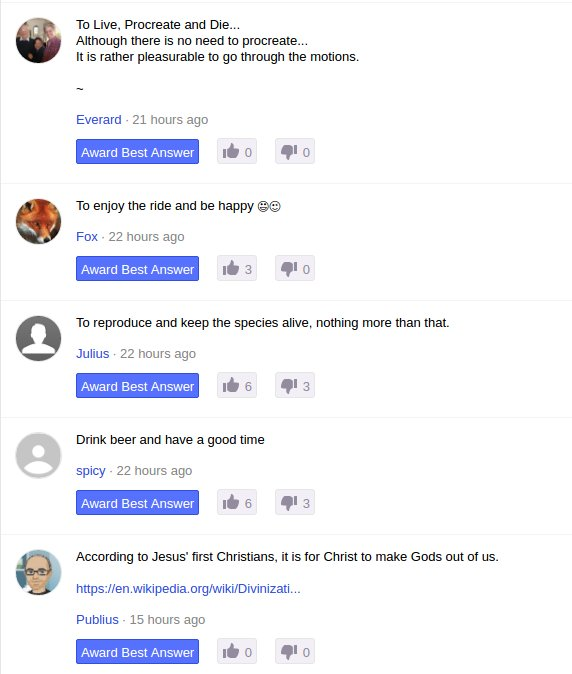
\includegraphics[scale=0.6]{10_5_a1}}
	\centering
	\caption{Answers for the low-quality question I asked on Yahoo Answers}
	\label{fig:10_5_a1}
\end{figure}

\begin{figure}[H]
	\fbox{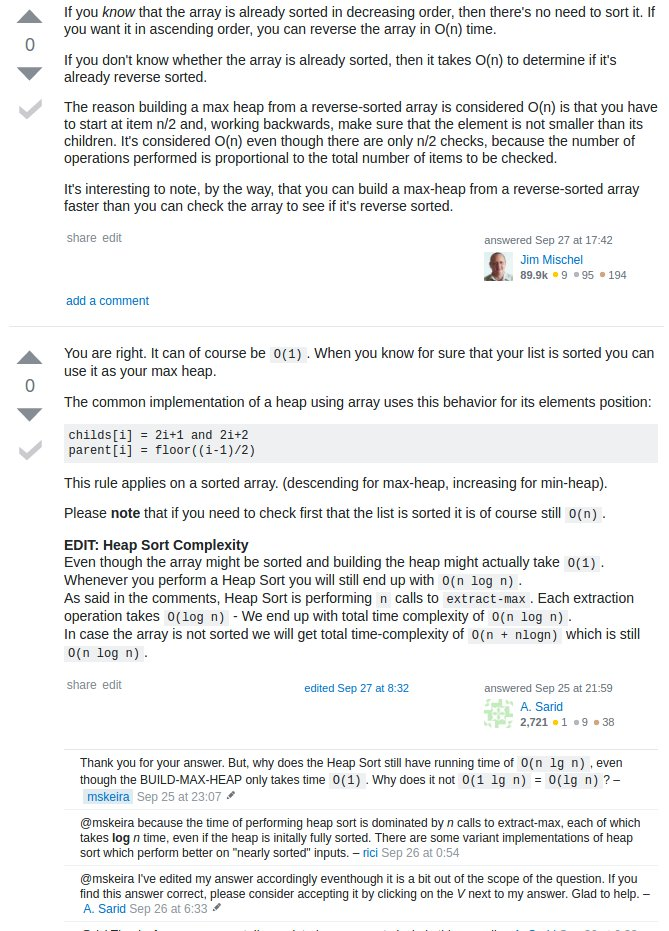
\includegraphics[scale=0.6]{10_5_high_quality_answer}}
	\centering
	\caption{Answers for the high-quality question I asked on Stackoverflow}
	\label{fig:10_5_high_quality_answer}
\end{figure}


\noindent\makebox[\linewidth]{\rule{\textwidth}{0.4pt}}

\section*{Question 10.6}
\begin{spverbatim}
Find two examples of document filtering systems on the Web. How do they build a profile for your information need? Is the system static or adaptive?
\end{spverbatim}

\subsection*{Answer}
I found 2 examples of document filtering systems on the Web, which are:
\begin{enumerate}
	\item Google Alerts (\url{https://www.google.com/alerts}). This is a content change detection and notification service, offered by the search engine company Google. 
	\item Twilert (\url{https://www.twilert.com/}). This is a tool to get realtime alerts anytime a certain keyword you are interested in are mentioned on Twitter. 
\end{enumerate}

Both Google Alerts and Twilert use the same method to build the profile: using input from the user. Figure \ref{fig:10_6_google_alerts} and \ref{fig:10_6_twilert_input} shows the creation of profile on Google Alerts and Twilert, respectively. \newline
To build a profile on Google Alerts, a user needs to input several information:
\begin{enumerate}
	\item The keyword that the user is interested in. This keyword will be the profile's name. 
	\item Sources: news, blogs, videos, etc
	\item Language: English, Arabic, etc
	\item Region: select a country's name
	\item How many: best results, all results. 
	\item Deliver to: user's email address. 
\end{enumerate}

\begin{figure}[H]
	\fbox{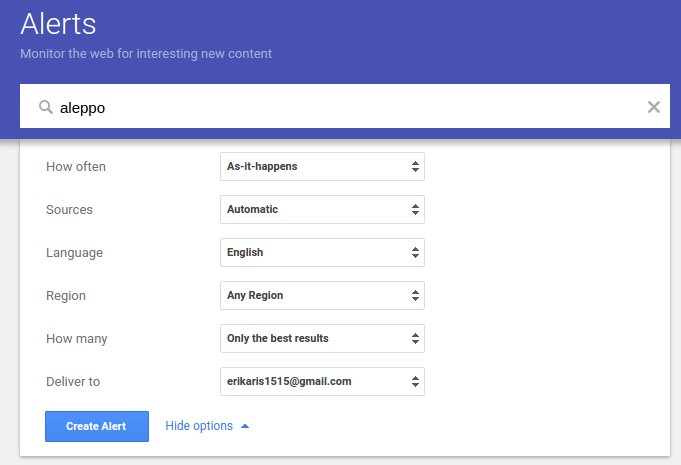
\includegraphics[scale=0.6]{10_6_google_alerts}}
	\centering
	\caption{Creating a profile on Google Alerts}
	\label{fig:10_6_google_alerts}
\end{figure}

Similarly, to build a profile on Twilert, user also needs to input several information such as the keyword, the location of the tweets, and the type of the tweets (positive, negative, or question). 

\begin{figure}[H]
	\fbox{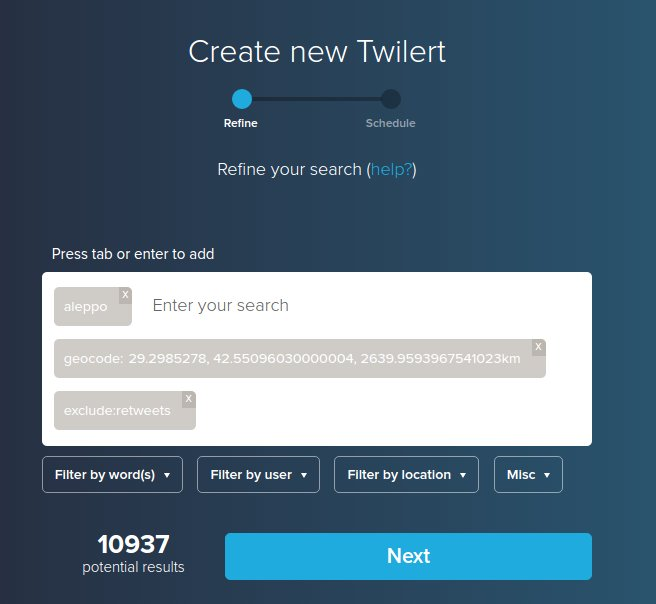
\includegraphics[scale=0.6]{10_6_twilert_input}}
	\centering
	\caption{Creating a profile on Twilert}
	\label{fig:10_6_twilert_input}
\end{figure}

The key to determine if a filtering system is static or adaptive is to check whether the profile is updateable or not. Based on this definition, I can conlude that both Google Alerts and Twilert are using adaptive filtering system since they provide a menu to update/edit profile. Figure \ref{fig:10_6_google_alert_edit} and \ref{fig:10_6_twilert_input_edit} illustrate the profile update for Google Alerts and Twilert, respectively. In this case, I make the keyword more specific by changing `aleppo' to `aleppo evacuation'. For Twilert, I also specify the tweet location to `Syria' (figure \ref{fig:10_6_twilert_area2}).

\begin{figure}[H]
	\fbox{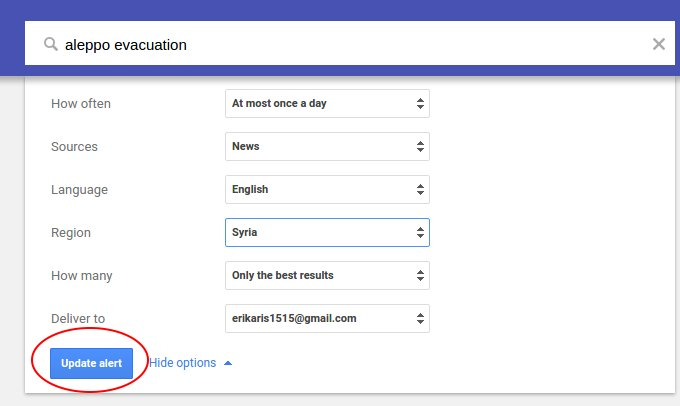
\includegraphics[scale=0.5]{10_6_google_alert_edit}}
	\centering
	\caption{Update a profile on Google Alerts}
	\label{fig:10_6_google_alert_edit}
\end{figure}

\begin{figure}[H]
	\fbox{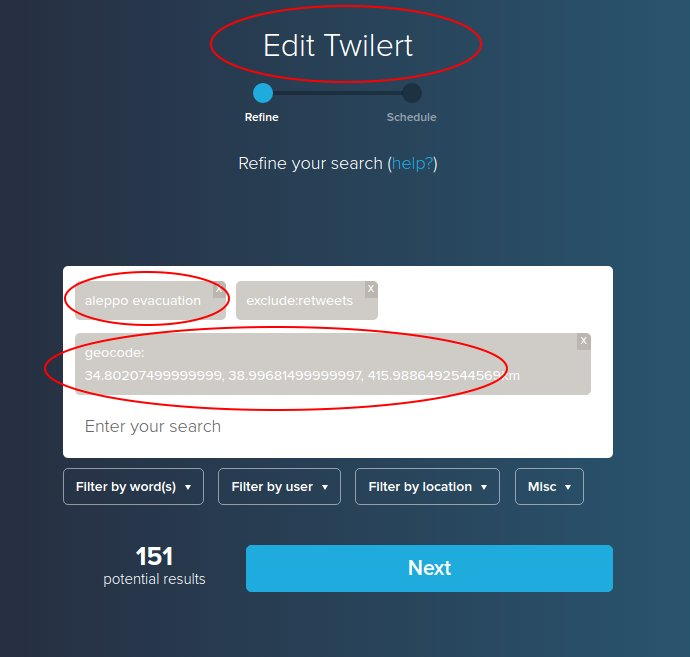
\includegraphics[scale=0.5]{10_6_twilert_input_edit}}
	\centering
	\caption{Update a profile on Twilert}
	\label{fig:10_6_twilert_input_edit}
\end{figure}

\begin{figure}[H]
	\fbox{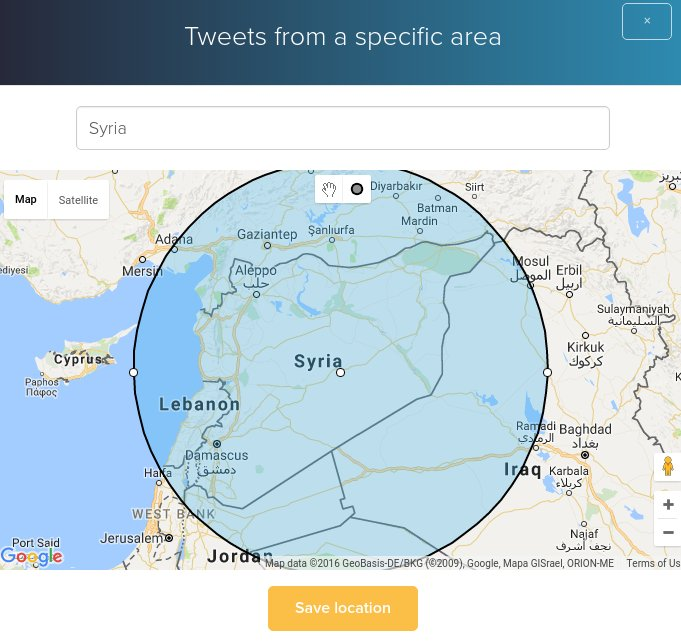
\includegraphics[scale=0.5]{10_6_twilert_area2}}
	\centering
	\caption{Update a profile on Twilert - update the area}
	\label{fig:10_6_twilert_area2}
\end{figure}

Figure \ref{fig:10_6_google_alerts_result} and \ref{fig:10_6_twilert_output} show the filtering result from Google Alerts and Twilert, respectively. 

\begin{figure}[H]
	\fbox{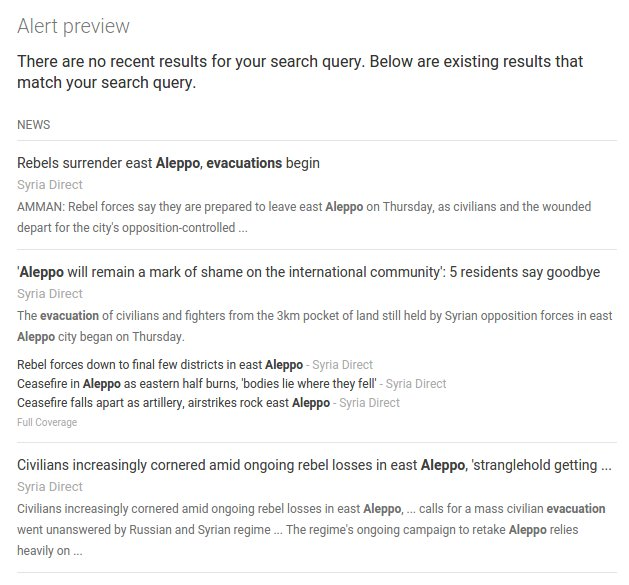
\includegraphics[scale=0.5]{10_6_google_alerts_result}}
	\centering
	\caption{Filter result by Google Alert}
	\label{fig:10_6_google_alerts_result}
\end{figure}

\begin{figure}[H]
	\fbox{
\includegraphics[scale=0.5]{10_6_twilert_output}}
	\centering
	\caption{Filter result by Twilert}
	\label{fig:10_6_twilert_output}
\end{figure}


\noindent\makebox[\linewidth]{\rule{\textwidth}{0.4pt}}

\section*{Question 7.5}
\begin{spverbatim}
Implement a BM25 module for Galago. Show that it works and document it.
\end{spverbatim}

\subsection*{Answer}
Information about how to impelemnt BM25 on Galago can be found on Lemur Project website \cite{galago-operators}. First, we have to make the json query file. The format for the json query is available on \cite{galago-operators} and it looks like the example on listing \ref{lst:query-bm25}.

\begin{lstlisting}[caption={json query format for BM25}, label={lst:query-bm25}]
	"queries" : [
	{
	"number" : "bm25-combine",
	"text" : "#combine(#bm25(international) #bm25(organized) #bm25(crime))",
	}
\end{lstlisting}

For this assignment, the json query that I use can be found on listing \ref{lst:query-bm25-me}.
\begin{lstlisting}[caption={json query format for BM25}, label={lst:query-bm25-me}]
	{
	"query": [
	{
	"text": "#combine(#bm25(what) #bm25(articles) #bm25(exist) #bm25(which) #bm25(deal) #bm25(with) #bm25(tss) #bm25(time) #bm25(sharing) #bm25(system) #bm25(an) #bm25(operating) #bm25(system) #bm25(for) #bm25(ibm) #bm25(computers))", 
	"number": "1"
	}
	]
	}
\end{lstlisting}


To execute this query, use the command \textbf{`./galago batch-search --index="[path to the index files]" --requested=10 [path to the json query]'}. Output of this execution is shown on figure \ref{fig:7_5_galago_bm25_output}.

\begin{figure}[H]
	\fbox{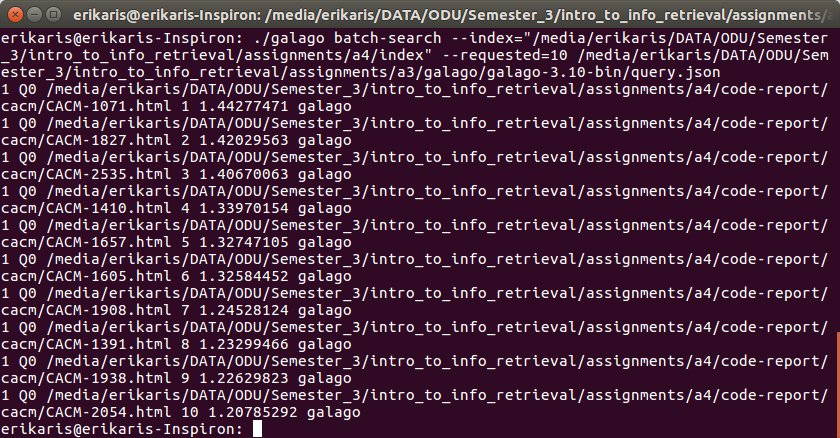
\includegraphics[scale=0.5]{7_5_galago_bm25_output}}
	\centering
	\caption{Output of BM25 implementation using Galago}
	\label{fig:7_5_galago_bm25_output}
\end{figure}


\noindent\makebox[\linewidth]{\rule{\textwidth}{0.4pt}}

\section*{Question 7.8}
\begin{spverbatim}
Using the Galago implementation of query likelihood, study the impact of short queries and long queries on effectiveness. Do the parameter settings make a difference?
\end{spverbatim}

\subsection*{Answer}
According to \cite{language-model}, the formula for query likelihood is what can be seen on figure \ref*{fig:7_8_likelihood_formula}.

\begin{figure}[H]
	\fbox{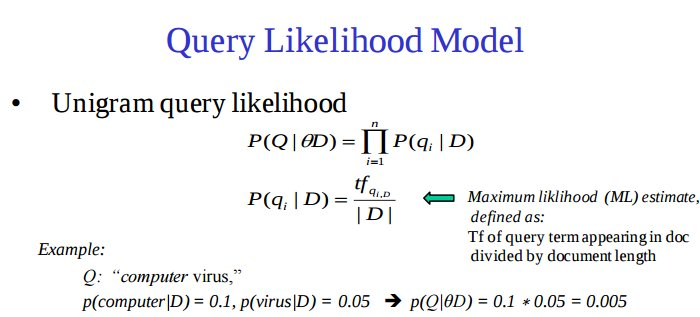
\includegraphics[scale=0.5]{7_8_likelihood_formula}}
	\centering
	\caption{Query Likelihood Formula}
	\label{fig:7_8_likelihood_formula}
\end{figure}

This formula has 2 drawbacks:
\begin{enumerate}
	\item Results in zero if a term is missing in document (figure \ref{fig:7_8_zero_problem})
	\item Document may be relevant to query but the query term is absent from document
\end{enumerate}


\begin{figure}[H]
	\fbox{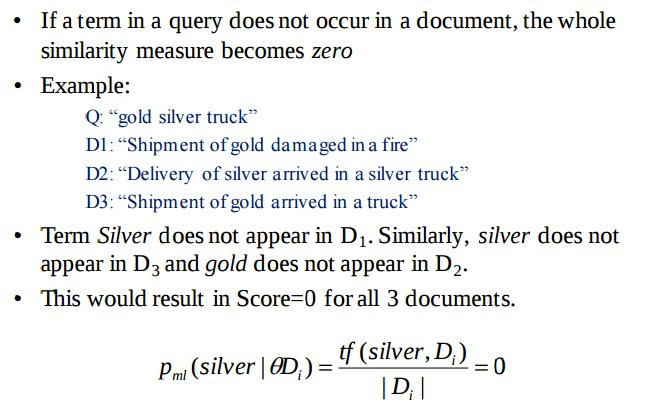
\includegraphics[scale=0.5]{7_8_zero_problem}}
	\centering
	\caption{Problem with missing document. Figure is taken from \cite{language-model}}
	\label{fig:7_8_zero_problem}
\end{figure}

To overcome these issues, smoothing is needed. By default, Galago uses DirichletScorer for smoothing \cite{galago-default-smoothing}. Figure \ref{fig:7_8_dirichlet} shows the snippet for DirichletScorer code that can be found in file `DirichletScoringIterator.java' line 56 in Galago Project. 

\begin{figure}[H]
	\fbox{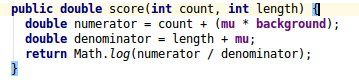
\includegraphics[scale=0.6]{7_8_dirichlet}}
	\centering
	\caption{Snippet for Dirichlet code in Galago Project}
	\label{fig:7_8_dirichlet}
\end{figure}

Using short query could impact the effectiveness since short query might contains noises (things that are not really relevant) in the result set. On the other hand, using a very long query could lower the likelihood value, especiallly if the long query contain a lower proportion of keywords. For example, the query `search engines' may produce a better result with a web search engine than the query `“what are typical implementation techniques and data structures used in search engines'. Therefore, the best thing to do is to use an average-length query since it has enough keywords to produce a good result, but contain less noise compare to the short query. \newline
Parameter setting (query, query format, input file format, output file format, etc) will have insignificant effect on the query effectiveness. It normally will not affect the top-ranked pages of the search engine result. 

\noindent\makebox[\linewidth]{\rule{\textwidth}{0.4pt}}


\section*{Question 10.8}
\begin{spverbatim}
Implement the nearest neighbor–based collaborative filtering algorithm. Using a publicly available collaborative filtering data set, compare the effectiveness, in terms of mean squared error, of the Euclidean distance and correlation similarity.
\end{spverbatim}

\subsection*{Answer}
For this assignment, I use the movielens dataset which is available at \url{http://grouplens.org/datasets/movielens/100k/}. I wrote a python program that utilize python libraries `scipy' and `sklearn'. The complete code can be found on listing \ref{lst:10_8}. \newline
Based on the output on figure \ref{fig:10_8} we can see that the MSE of Euclidean distance is smaller than the MSE of the correlation similarity (Pearson). Therefore, in this case, we can conclude that Euclidean distance is more effective compare to correlation similarity (Pearson). 

\begin{figure}[H]
	\fbox{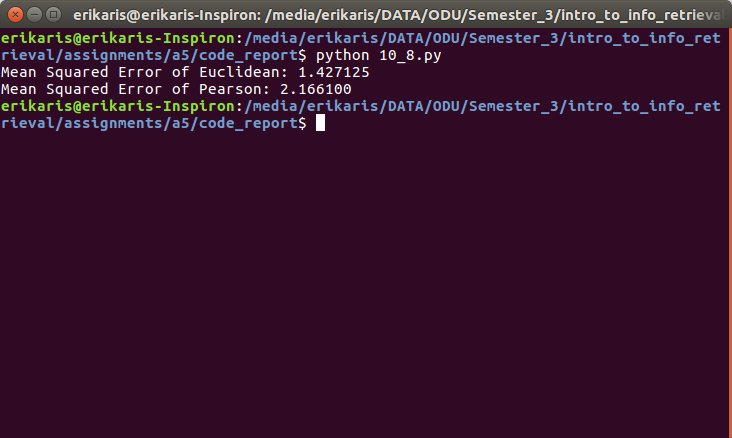
\includegraphics[scale=0.6]{10_8}}
	\centering
	\caption{Output for question 10\_8}
	\label{fig:10_8}
\end{figure}

\begin{lstlisting}[language=python, caption={Code for nearest neighbor–based collaborative filtering algorithm }, label={lst:10_8}]

#!/usr/bin/python
from numpy import genfromtxt, array, random
from sklearn.linear_model import LinearRegression
from sklearn.metrics import mean_squared_error
from sklearn.neighbors import KNeighborsClassifier

if __name__ == '__main__':
# Read data ratings.csv from movielens
ratings = genfromtxt('ratings.csv', delimiter=',', skip_header=1, usecols=range(3))

# Split data to train and test data, with ratio train:test = 0.9:0.1
random.shuffle(ratings)
train, test = ratings[len(ratings)/10:, :], ratings[:len(ratings)/10, :]

# Train data using KNN, get 1st top neighbor
neigh = KNeighborsClassifier(n_neighbors=1)
# X = 2-dimensional array, y = target = 1st col of X
neigh.fit(train, train[:, 0])
# Get neighbors indices (2-dimensional array)
distances, neighbors_indices = neigh.kneighbors(test)
# Get ratings from indices
euclidean_neighbors = array([train[ns[0]] for ns in neighbors_indices])

# Train data using Pearson
lr = LinearRegression()
# X = 2-dimensional array, y = target = 1st col of X
lr.fit(train, train[:, 0])
# Get neighbors index (1-dimensional array)
neighbors_idx = lr.predict(test)
# Get ratings from indices
pearson_neighbors = array([train[int(idx)] for idx in neighbors_idx])

# Get MSE of predicted ratings, for both euclidean and pearson
y_true = []
for user, movie, rating in test:
y_true.append(rating)

y_pred_euc = []
for user, movie, rating in euclidean_neighbors:
y_pred_euc.append(rating)

y_pred_pear = []
for user, movie, rating in pearson_neighbors:
y_pred_pear.append(rating)

print "Mean Squared Error of Euclidean: %f" % mean_squared_error(y_true, y_pred_euc)
print "Mean Squared Error of Pearson: %f" % mean_squared_error(y_true, y_pred_pear)


\end{lstlisting}

\noindent\makebox[\linewidth]{\rule{\textwidth}{0.4pt}}


\medskip

\bibliographystyle{unsrt}%Used BibTeX style is unsrt
\bibliography{biblio}

\end{document}
